\documentclass{beamer}
\usetheme{metropolis}
\usepackage{graphicx}
\usepackage{subfigure}
\usepackage{hyperref}
\usepackage{tcolorbox}
\title{Algebra-Based Physics-1: Mechanics (PHYS135A-01): Week 7}
\date{October 16th - October 20th, 2017}
\author{Jordan Hanson}
\institute{Whittier College Department of Physics and Astronomy}

\begin{document}
\maketitle

\section{Week 6 Review}

\begin{frame}{Week 6 Review}
\begin{enumerate}
\item \alert{Angular} kinematics and dynamics
\begin{itemize}
\item Angular displacement
\item Angular velocity
\item Centripetal acceleration
\end{itemize}
\item \alert{Newton's Law of Gravity} and circular orbits
\item Kepler's Laws
\end{enumerate}
\end{frame}

\section{Week 6 Review Problem}

\begin{frame}{Week 6 Review Problem}
On the game show Wheel of Fortune, a large wheel is divided into sections worth varying dollar amounts.  Contestants try to spin the wheel such that they get the good ones.  Player 1 notices that the \$10,000 marker is on the opposite side (180 degrees away).  What is this angle in radians?  If she has great luck and spins such that the wheel turns exactly 180 degrees, in 2 seconds, what is the angular speed in radians per second?
\begin{itemize}
\item A: $\pi/2$ radians, $\pi/4$ radians per second
\item B: $0$ radians, $0$ radians per second
\item C: $\pi$, $\pi/2$ radians per second
\item D: $\pi$, $\pi/4$ radians per second
\end{itemize}
\end{frame}

\begin{frame}{Week 6 Review Problem}
Astronomers are observing two planets orbiting a star for several months.  They observe that planet 1 orbits twice as fast as planet 2.  If the orbital radius of planet 1 is 1 AU, what is the orbital radius of planet 2, in AU?
\begin{itemize}
\item A: 1 AU
\item B: 1.6 AU
\item C: 4 AU
\item D: 3.2 AU
\end{itemize}
\end{frame}

\section{Week 7 Summary}

\begin{frame}{Week 7 Summary}
\begin{enumerate}
\item \alert{Work} has a scientifically precise definition
\begin{itemize}
\item Units
\item As a product of force and displacement vectors
\end{itemize}
\item Kinetic Energy and the \alert{Work-Energy Theorem}
\item Gravitational potential energy
\begin{itemize}
\item Potential energy
\item \textit{Simplifying otherwise complex calculations}
\item Potential energy near Earth's surface
\item ...in space
\end{itemize}
\item Definition of a \textbf{conservative force}
\begin{itemize}
\item Relationship between conservative forces and potential energy
\item Conservation of energy for conservative forces
\end{itemize}
\end{enumerate}
\end{frame}

\section{Definitions of Work}

\begin{frame}{Definitions of Work}
\begin{tcolorbox}[colback=white,colframe=red!40!blue,title=Physical Definition of Work]
\alert{Let $\vec{F}$ be a force exerted on a system, which is displaced by a displacement $\vec{x}$.  The \textbf{work} done on the system is} \\
\alert{$W = \vec{F} \cdot \vec{x}$} \\
\end{tcolorbox}
The units of work are N m, or \textit{Joules}. \\
\textit{Extra credit opportunity}: \textbf{Do you like beer}?  Write a 10-page paper on the on the scientific challenge faced by James Prescott Joule, who began to formulate the modern view of energy in the 19th century, contrary to the prior paradigm (\textit{caloric theory}).
\end{frame}

\begin{frame}{Definitions of Work}
Let $\theta$ be the angle between the force and the displacement.  Then this equation
\begin{equation}
W = \vec{F} \cdot \vec{x}
\end{equation}
becomes
\begin{equation}
W = Fx\cos\theta
\end{equation}
\end{frame}

\begin{frame}{Definitions of Work}
\begin{figure}
\centering
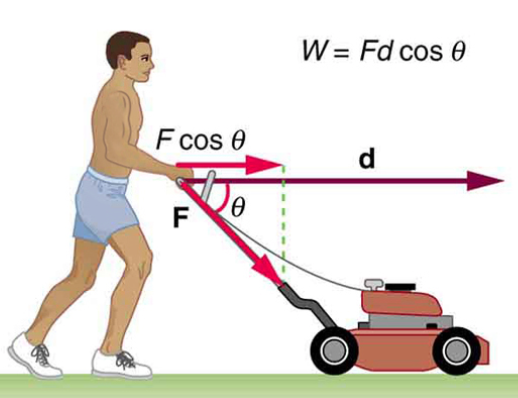
\includegraphics[width=0.7\textwidth]{figures/lawn.png}
\caption{\label{fig:work} A case where $\theta \neq 0$.}
\end{figure}
\end{frame}

\begin{frame}{Definitions of Work}
\begin{figure}
\centering
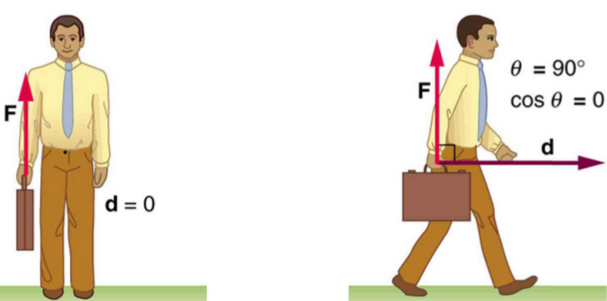
\includegraphics[width=0.8\textwidth]{figures/lawn2.png}
\caption{\label{fig:work2} (Left): A case where $x = 0$, so $W=0$.  (Right): A case where $\theta = 90^{\circ}$, so $W=0$.}
\end{figure}
\end{frame}

\section{Conclusion}

\begin{frame}{Week 7 Summary}
\begin{enumerate}
\item \alert{Work} has a scientifically precise definition
\begin{itemize}
\item Units
\item As a product of force and displacement vectors
\end{itemize}
\item Kinetic Energy and the \alert{Work-Energy Theorem}
\item Gravitational potential energy
\begin{itemize}
\item Potential energy
\item \textit{Simplifying otherwise complex calculations}
\item Potential energy near Earth's surface
\item ...in space
\end{itemize}
\item Definition of a \textbf{conservative force}
\begin{itemize}
\item Relationship between conservative forces and potential energy
\item Conservation of energy for conservative forces
\end{itemize}
\end{enumerate}
\end{frame}

\section{Answers}

\begin{frame}{Answers}
\begin{columns}[T]
\begin{column}{0.5\textwidth}
\begin{itemize}
\item $\pi$, $\pi/2$ radians per second
\item 1.6 AU
\end{itemize}
\end{column}
\begin{column}{0.5\textwidth}
\begin{itemize}
\item ... 
\end{itemize}
\end{column}
\end{columns}
\end{frame}

\end{document}
